\section{Benchmarks}
\label{sec:benchmarks}

Dans cette section nous présentons différents résultats obtenus en faisant varier les paramètres du système.
On peut classer ces paramètres en deux catégories principales:\\

\begin{itemize}
\item Paramètres des agents : champs de vision, temps avant message\footnote{Combien de temps avant de sortir d'une place un agent envoi un message}, temps avant recherche\footnote{Combien de temps après être sorti d'une place un agent commence à en rechercher une autre}, temps resté sur une place
\item Paramètres du système : nombre d'agents, nombre de places\\
\end{itemize}

Chacun de ces paramètres (des agents ou du système) influence directement les résultats de notre méthode.
On s'aperçoit ainsi qu'elle est robuste face à la variation de certains et non robuste par rapport à d'autre.\\

Pour chacun de ces paramètres nous mesurons trois indicateurs différents:\\

\begin{itemize}
\item Nombre de messages totaux envoyés
\item Pourcentage du temps passé à chercher aléatoirement une place par rapport au temps passé à se déplacer vers une place.
\item Ratio temps garé par rapport au temps total de la simulation\\
\end{itemize}

Ces indicateurs nous semblent les plus importants car ils décrivent la consommation du système (nombre de message) et sa performance.
Cette dernière possède deux aspects : La qualité de la place trouvé par l'agent (le pourcentage, fonction de la distance) qui traduit une 
performance local du système pour chaque agent. Et le temps total passé garé qui est une performance globale du système.

\subsection{Paramètres des agents}

Lors de ces tests nous ne faisons varier qu'un seul paramètre. Tous les autres prennent leurs valeurs par défaut:\\

\begin{itemize}
\item Nombre d'agents : 200
\item Nombre de places : 100
\item Champs de visions : 10
\item Temps avant message : 3
\item Temps avant recherche : 10
\item Temps resté sur une place : 10\\
\end{itemize}

Pour cette configuration on a les valeurs suivantes :\\

\begin{itemize}
\item Nombre de messages totaux envoyés :
\item Pourcentage temps de recherche / temps vers place : 
\item Pourcentage temps garé / temps total :
\end{itemize}

\subsubsection{Variations du champs de visions}

Dans un premier temps nous faisons varier le champs de vision de chaque agent entre 1 et 20 cases.

\paragraph{Résultats et Interpretation}

Les résultats sont présentés dans la figure \ref{vision:all}.

On remarque que logiquement, quand le champs de vision des agents augmente, ils détectent et signalent plus de placent et ainsi le nombre de messages envoyés augmente.
Cette augmentation se fait proportionnellement à la taille du champ de vision, ce qui s'explique par la répartition des places sur la grille. Avec un ratio voitures / places plus fort cette augmentation pourrait être plus importante.\\

On voit que notre système fonctionne bien en observant la décroissance du ratio vagabondage / vers place qui traduit la qualité de la place sélectionnée. Cette qualité s'améliore avec l'augmentation du champs de vision, ce qui prouve que malgré le nombre de place repéré l'agent prend généralement la plus proche.

La courbe du ratio total de temps garé s'explique par plus de places détectées et une qualité des solutions choisies qui s'améliore.

\begin{figure}
  \begin{center}
    \subfigure[Nombre de messages en fonction du champs de vision]{
      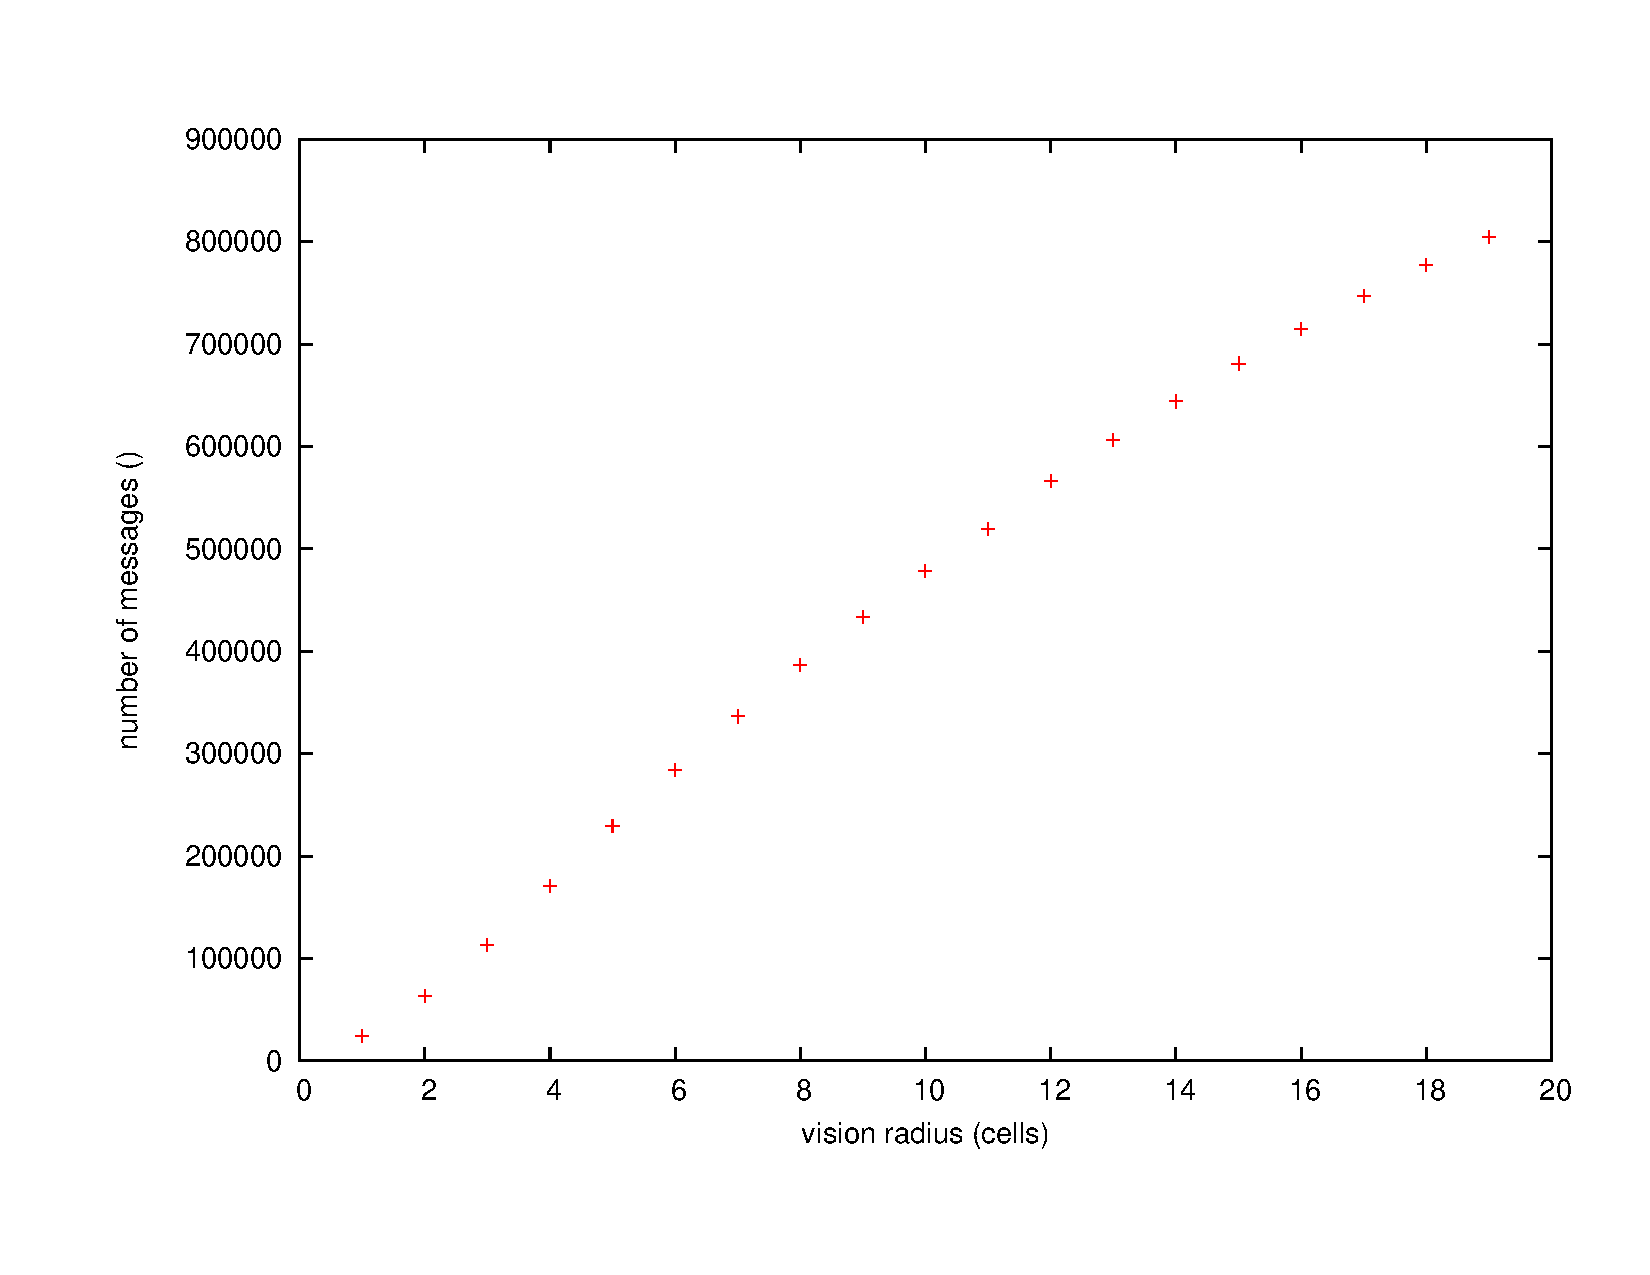
\includegraphics[scale=.3]{src/vision-message}
      \label{vision:message}
    }
    
    \subfigure[Pourcentage temps de vagabondage / temps vers place]{
      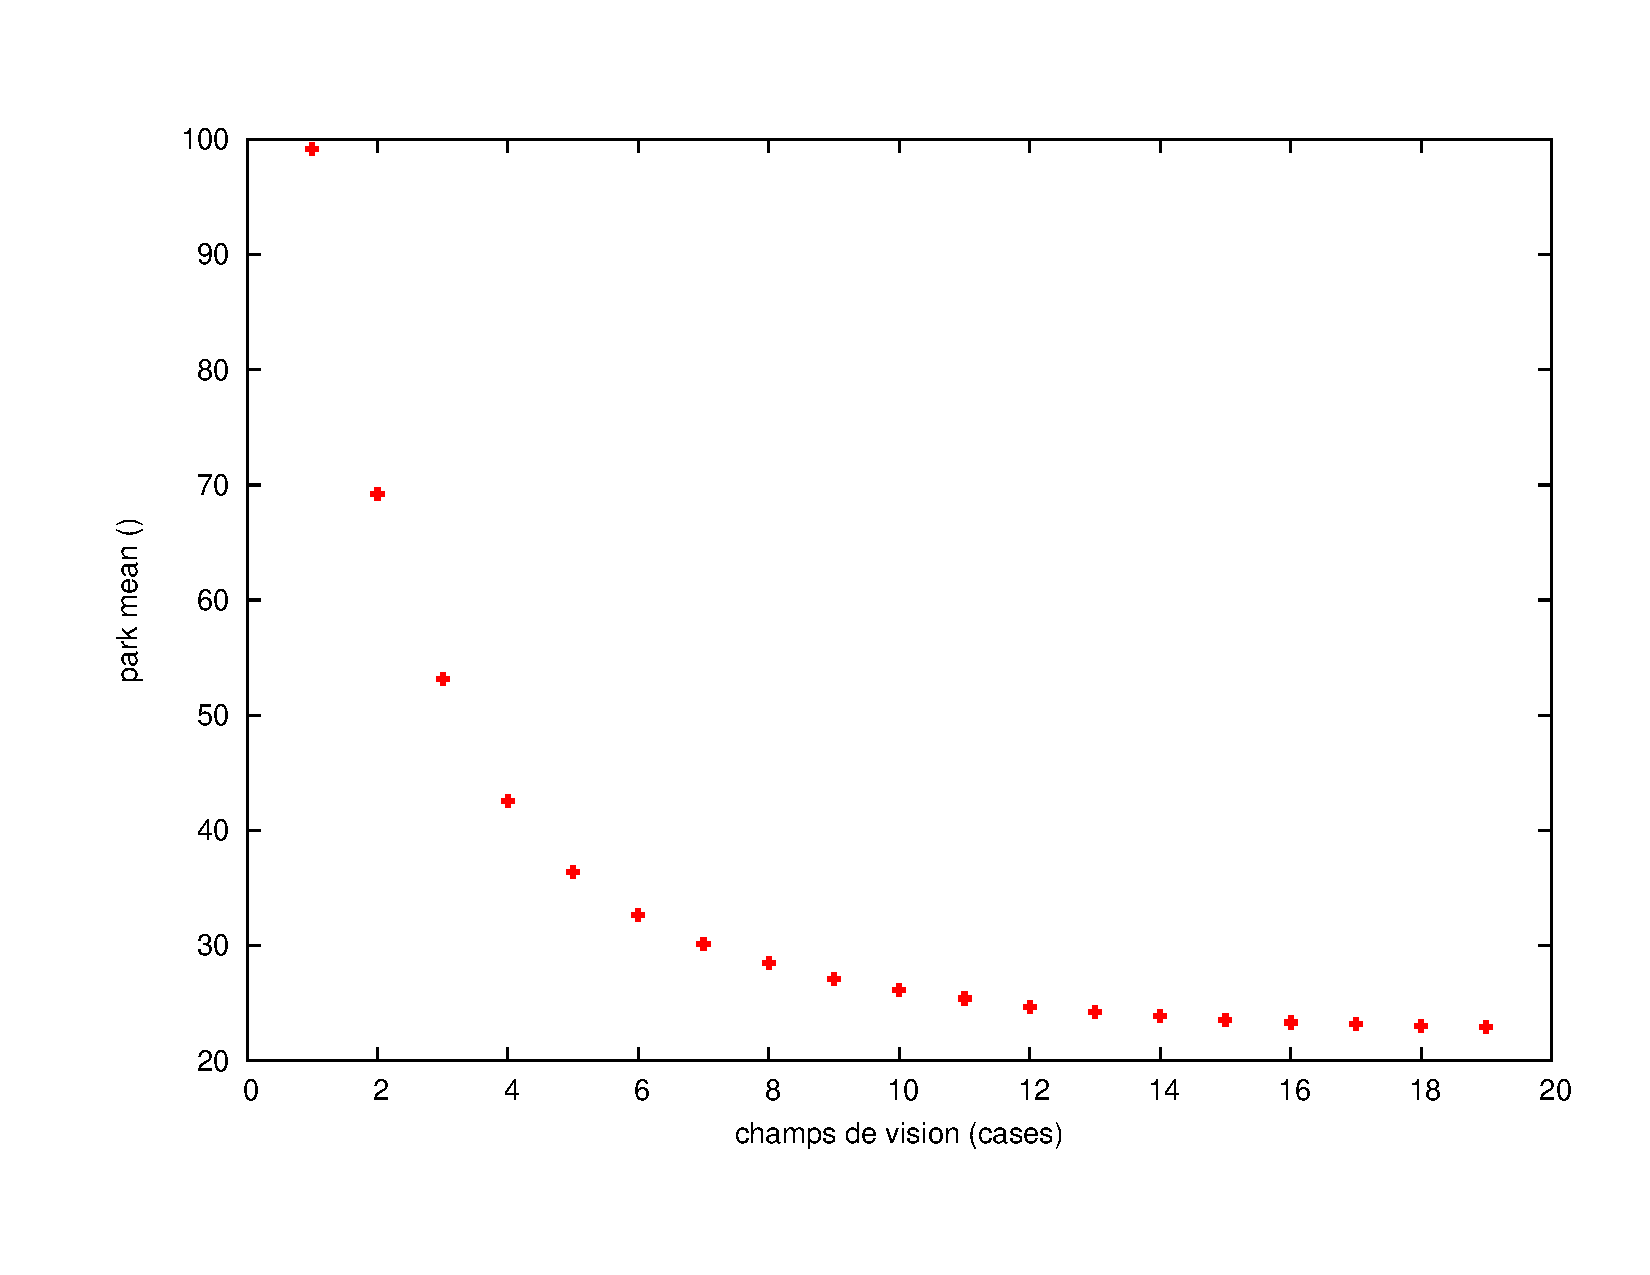
\includegraphics[scale=.3]{src/vision-seekfound}
      \label{vision:seekfound}
    }
    
    \subfigure[Ratio temps garé / temps total]{
      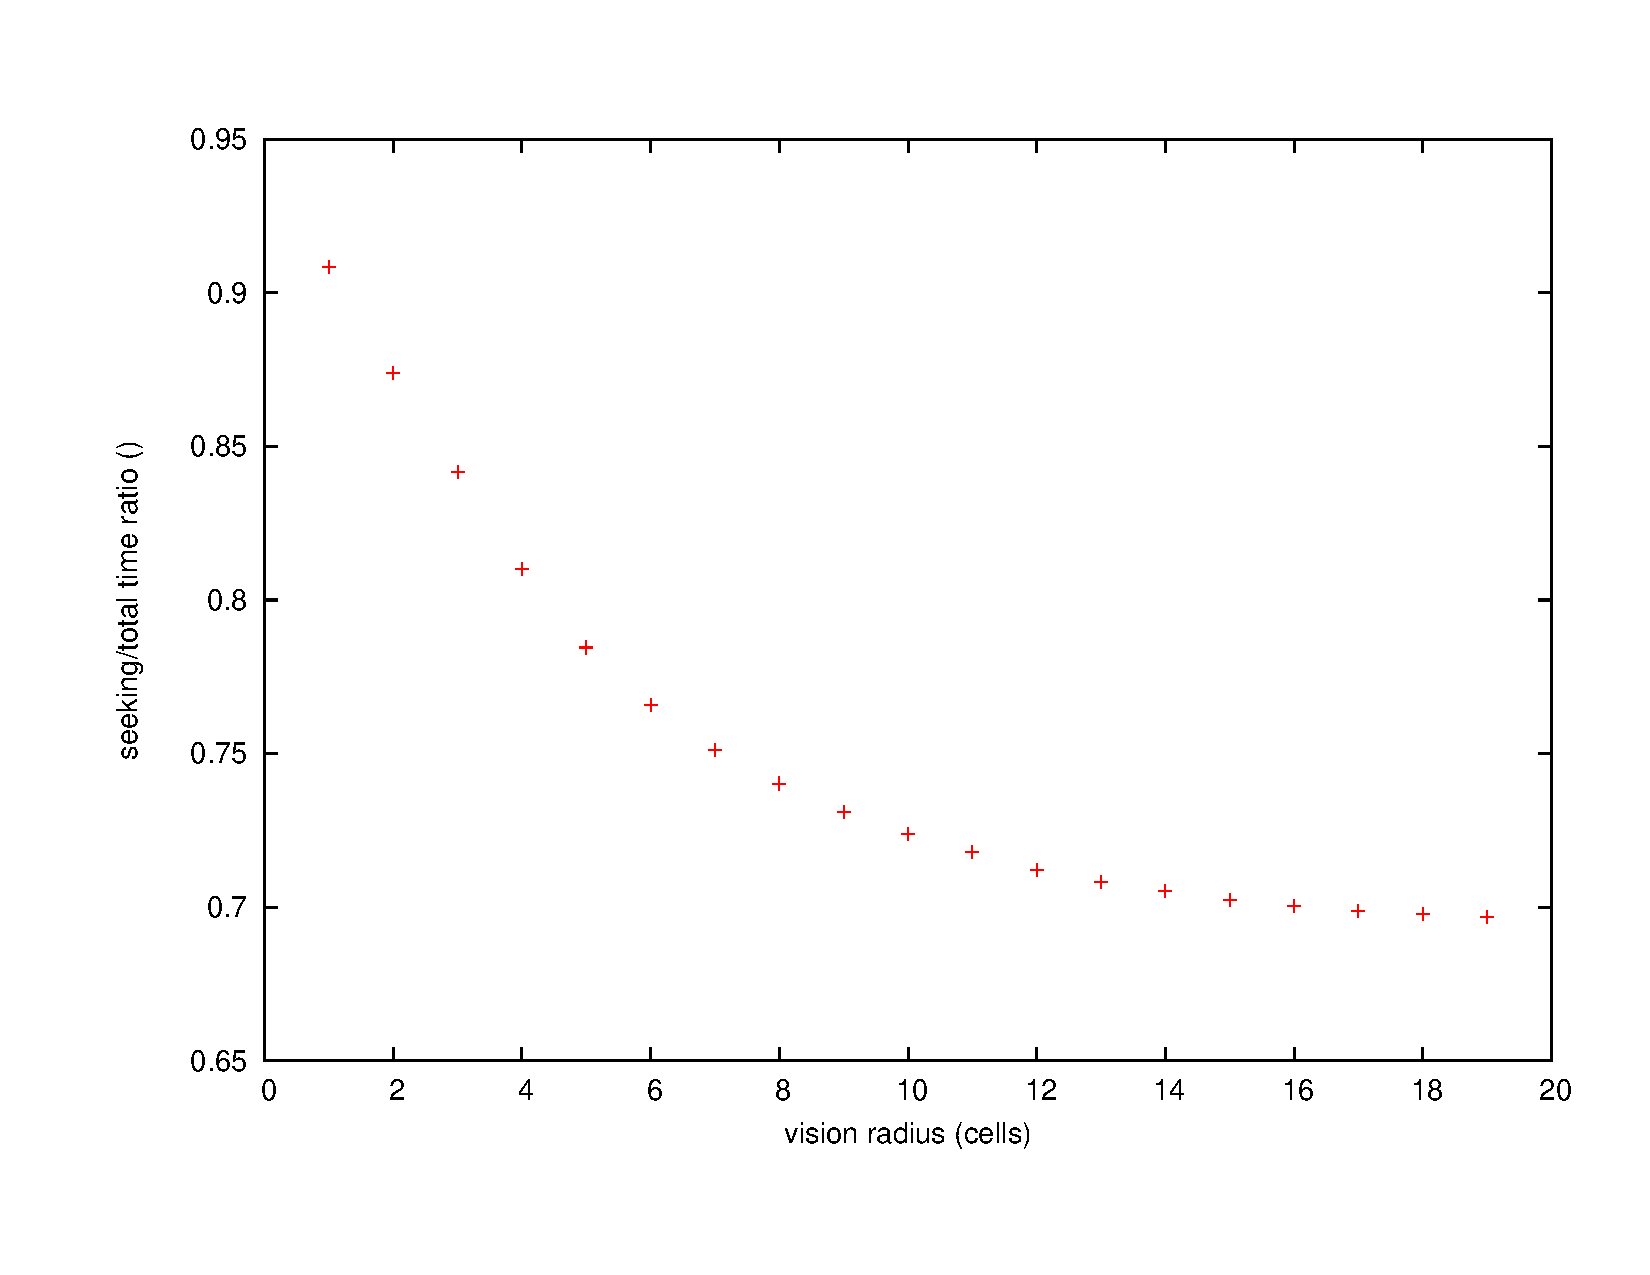
\includegraphics[scale=.3]{src/vision-seeking}
      \label{vision:seeking}
    }
  \end{center}

  \caption{Résultats obtenus en faisant varier le champs de visions}
  \label{vision:all}
\end{figure}

\subsubsection{Variation du temps de stationnement}

Deuxième paramètre à varier, le temps de stationnement, entre 0 et 15 rounds.

\paragraph{Résultats et interprétation}

Les résultats sont présentés dans la figure \ref{parktime:all}
Le nombre de messages n'est pas vraiment influencé par le temps de stationnement.
En revanche on que plus le temps de stationnement est long, plus la qualité de la solution trouvé par chaque agent se dégrade. Ceci s'explique par le fait que vu qu'il y a deux fois moins de places que de voitures, les places libres deviennent de plus en plus rares. Encore une fois avec d'autres paramètres par défaut cette courbe changerait. En l'état elle illustre bien un processus de famine et à l'inverse quand le temps de stationnement est faible, les solutions sont de meilleur qualité.\\

Enfin la solution générale s'améliore grandement (plus qu'avec le champs de vision) avec un temps de stationnement plus long. Ceci est la combinaison du temps de stationnement long améliorant le ratio et du phénomène de raréfaction des ressources l'améliorant encore plus.\\

Ce paramètres montre bien la dualité qu'il y a entre qualité globale de la solution du système et la qualité locale des solutions choisies par chaque agents.

\begin{figure}
  \begin{center}
    \subfigure[Nombre de messages en fonction du temps de stationnement]{
      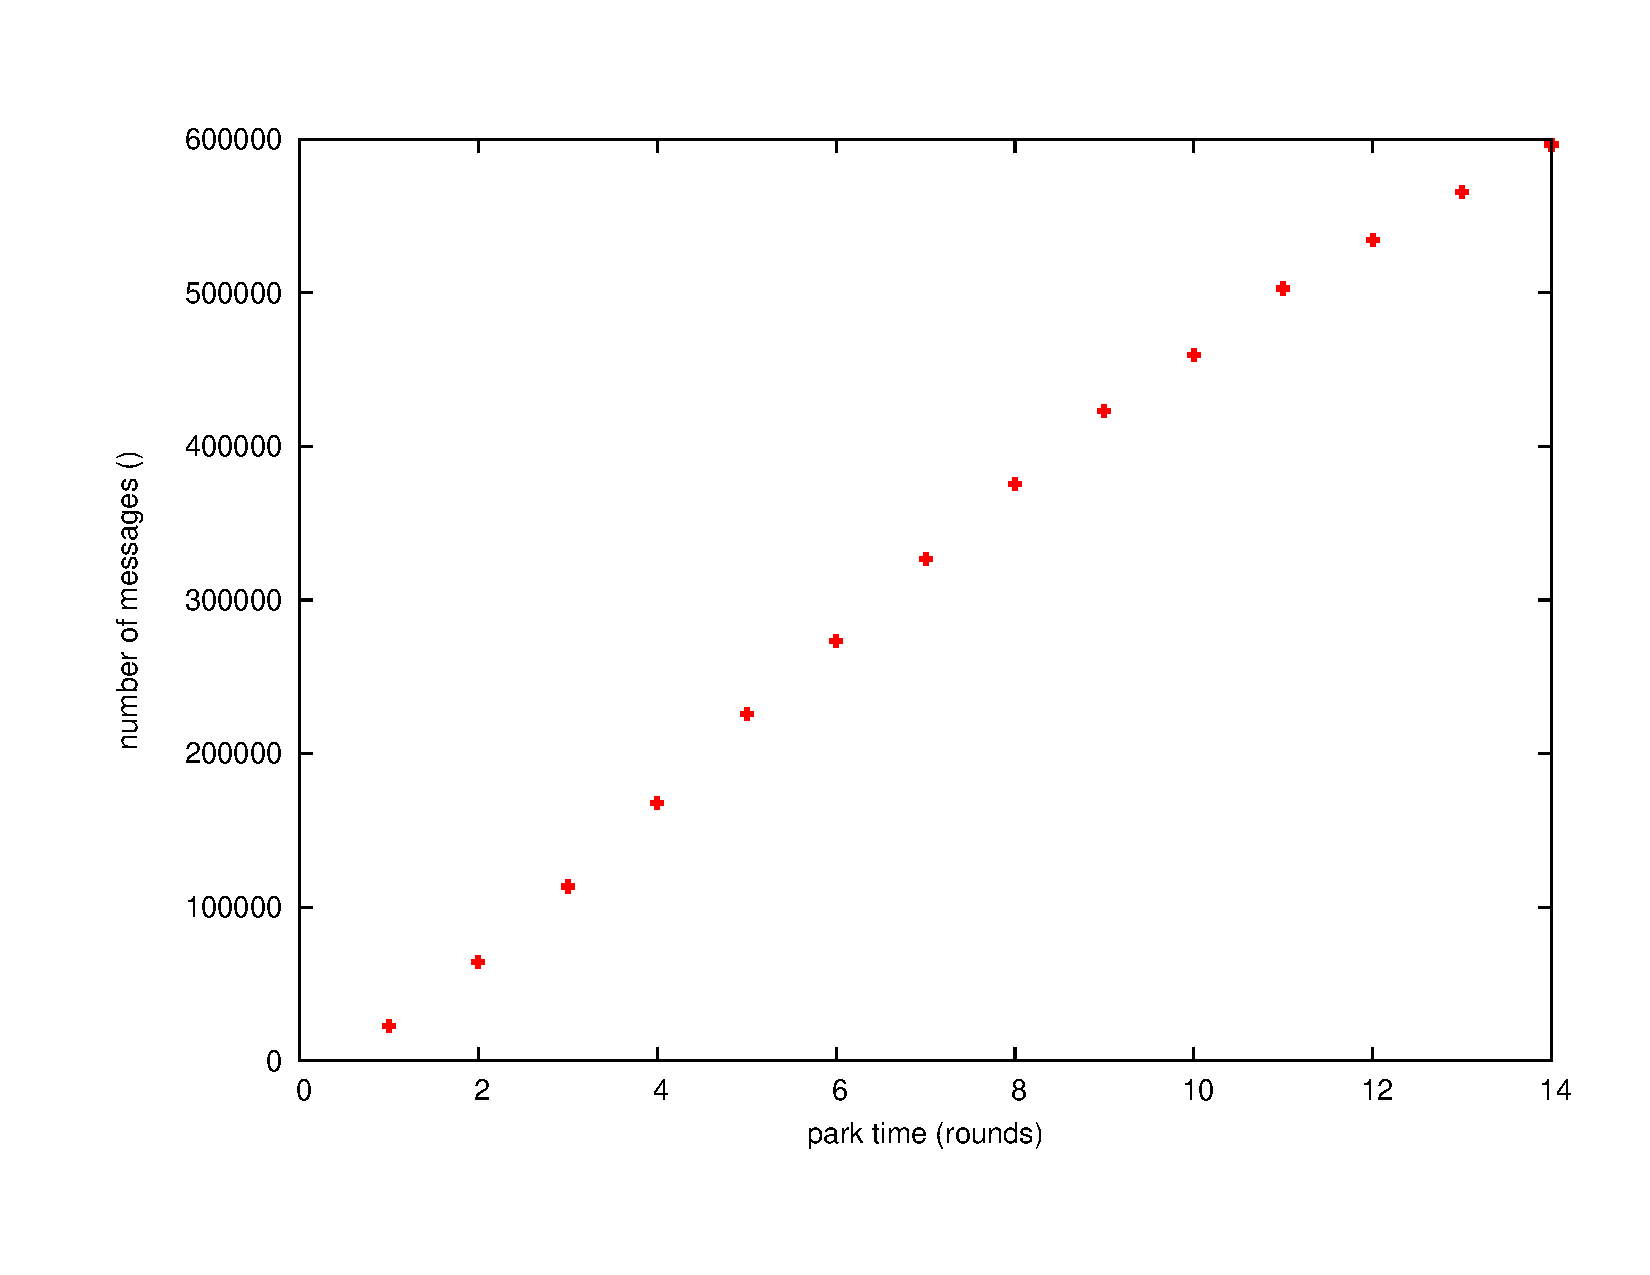
\includegraphics[scale=.3]{src/parktime-message}
      \label{parktime:message}
    }
    
    \subfigure[Pourcentage temps de vagabondage / temps vers place]{
      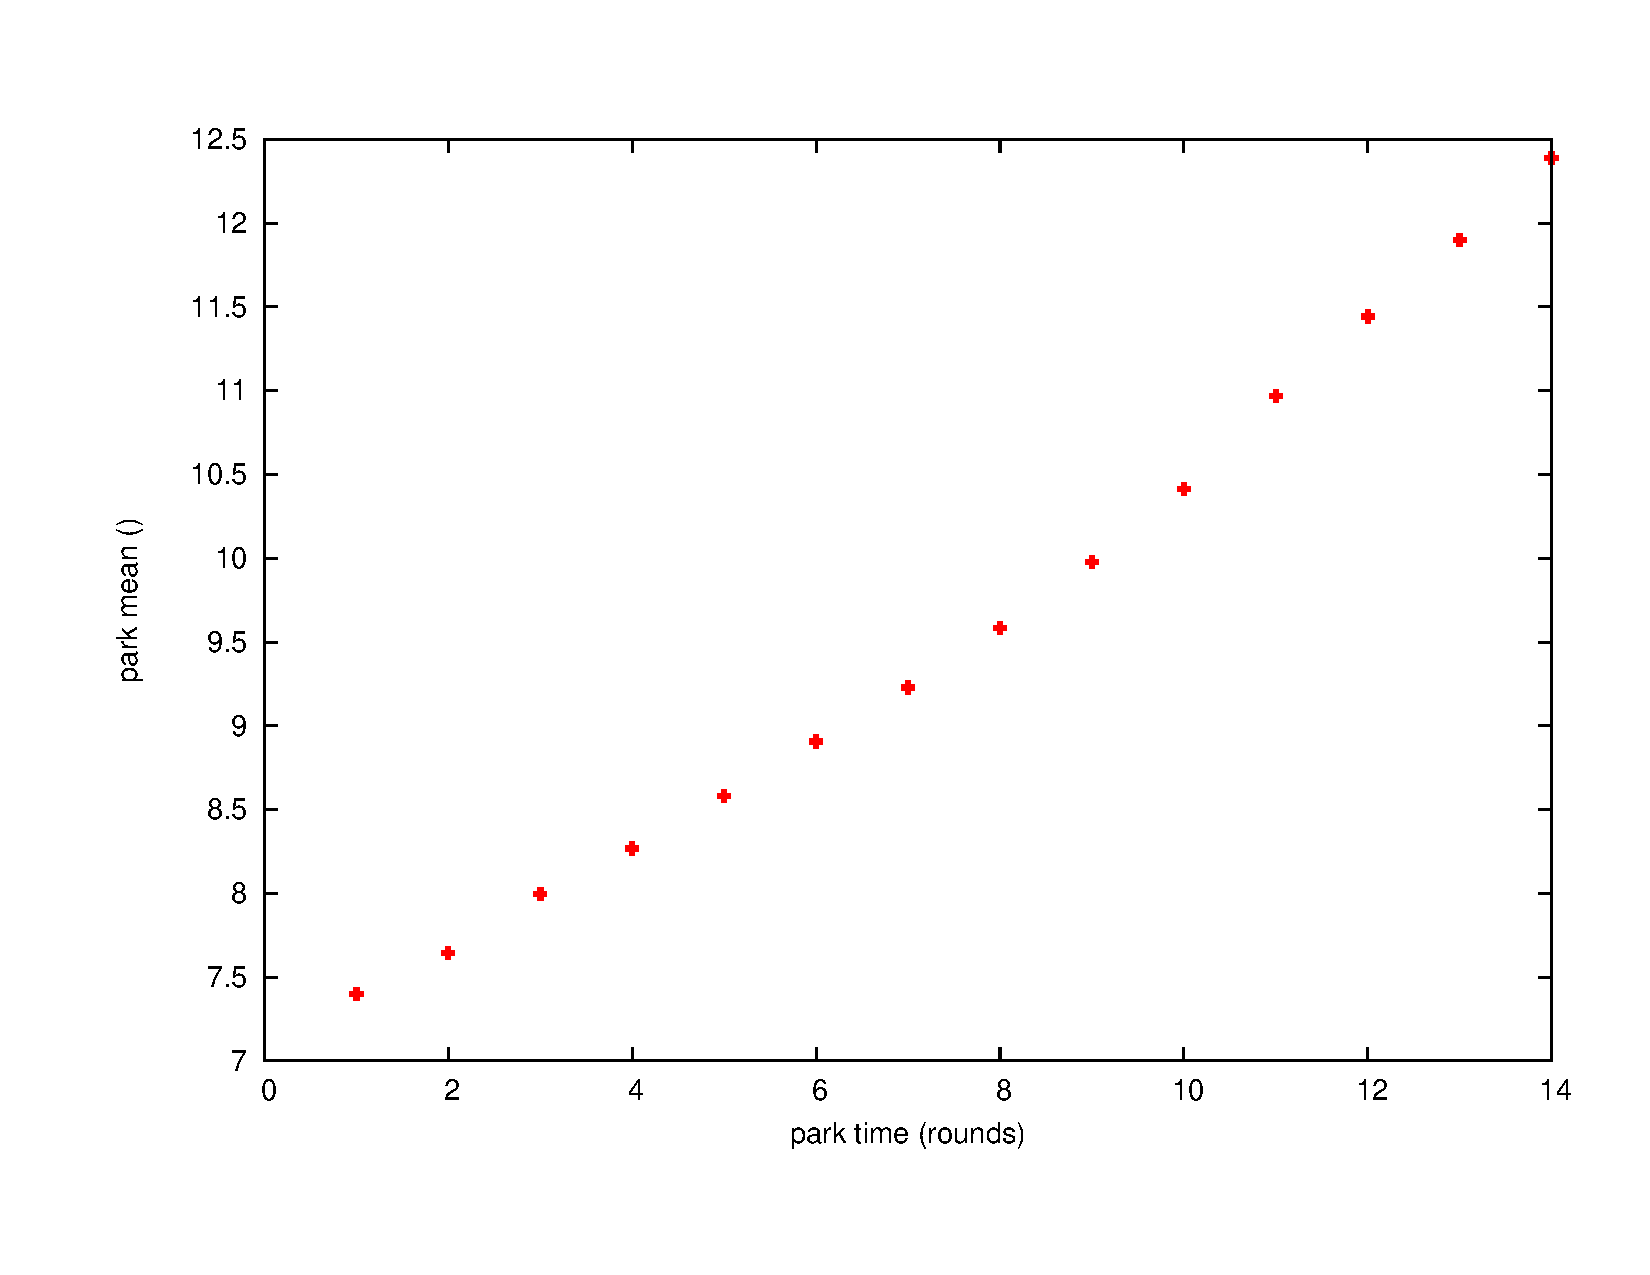
\includegraphics[scale=.3]{src/parktime-seekfound}
      \label{parktime:seekfound}
    }
    
    \subfigure[Ratio temps garé / temps total]{
      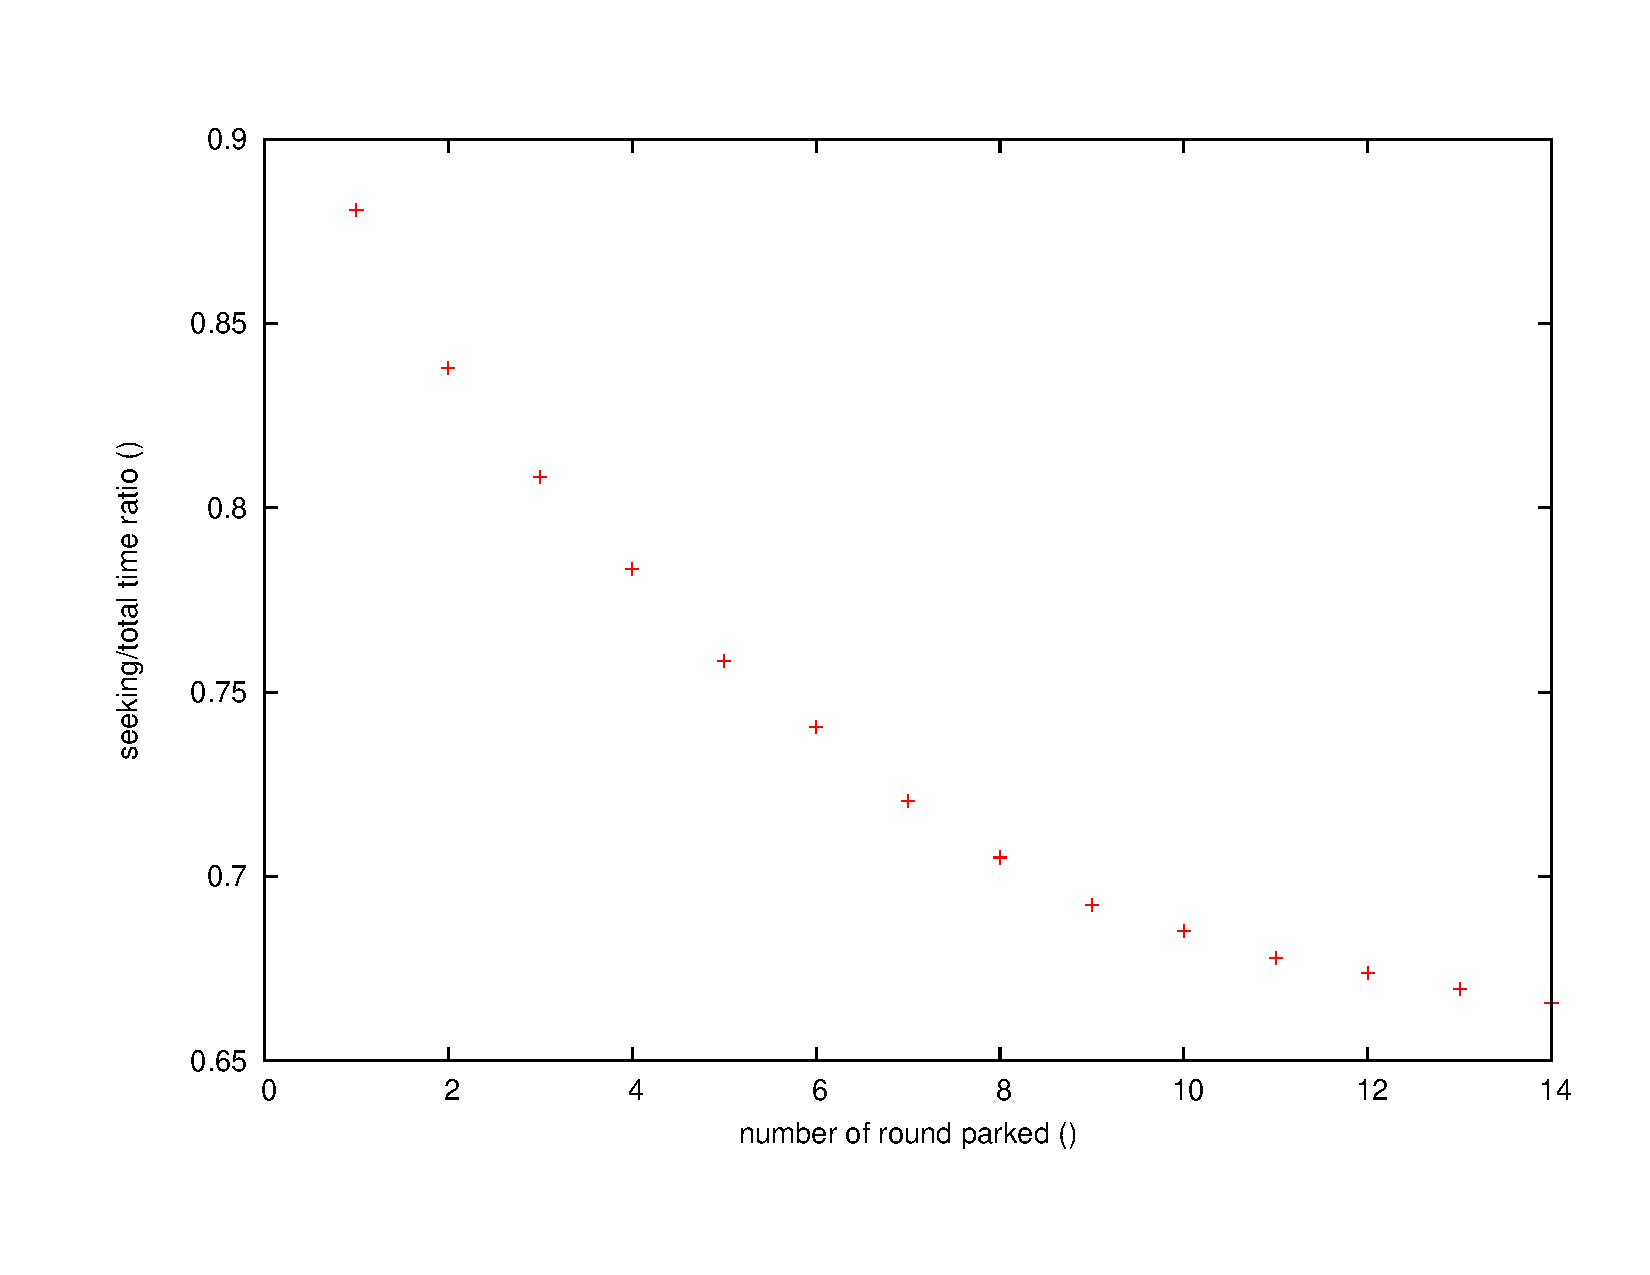
\includegraphics[scale=.3]{src/parktime-seeking}
      \label{parktime:seeking}
    }
  \end{center}

  \caption{Résultats obtenus en faisant varier le temps de stationnement}
  \label{parktime:all}
\end{figure}

\subsubsection{Temps de stationnement avant diffusion d'information}

Ce paramètre est spécifique à notre solution, c'est le nombre de rounds avant la fin du stationnement a partir duquel on va commencer à signaler que la place va se libérer. Ce temps est donné en nombre de rounds avant la fin du stationnement, entre 1 et 10.


\paragraph{Résultats et interprétation}

Les résultats sont présentés dans la figure \ref{timeb4broad:all}\\

{\bf Note: } Plus le temps avant diffusion est faible, plus l'agent va prévenir tard avant de quitter sa place. Ainsi avec un temps de 1 round l'agent prévient les autres 1 round avant de quitter sa place.\\

L'augmentation du nombre de messages envoyés s'explique simplement par le fait qu'à chaque round encore sur une place si il a commencé à diffuser l'agent continue à le faire. Plus il diffuse tard moins de messages sont donc envoyés. C'est le paramètre influençant le plus le nombre de messages transmis.\\

Par contre, plus les autres agents sont prévenus tard, moins il ont le temps de réagir donc plus la qualité locale et totale des solutions décroît. A noter quand même que la solution globale s'améliore plus que la solution locale quand le paramètre varie. Cela peut être du au phénomène de rarification des ressources propre à notre système.


\begin{figure}
  \begin{center}
    \subfigure[Nombre de messages en fonction du temps avant diffusion]{
      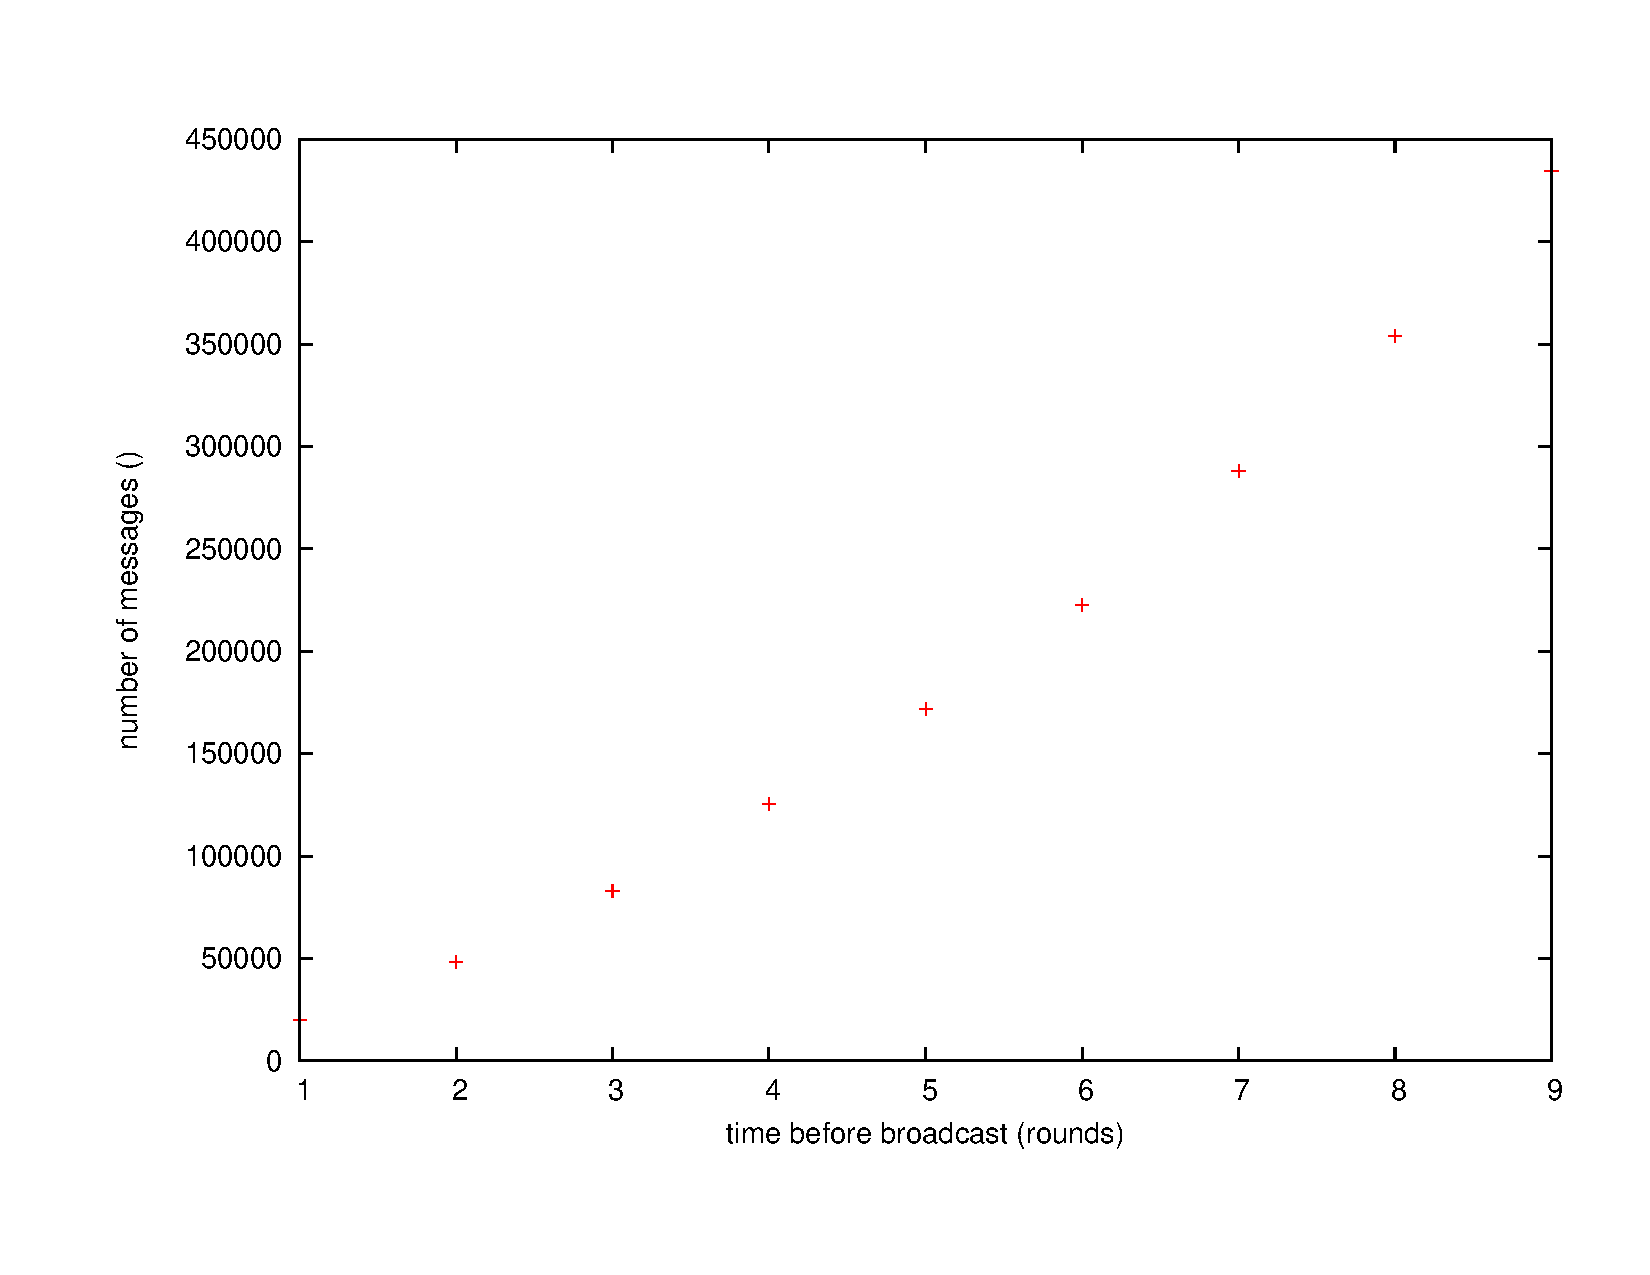
\includegraphics[scale=.3]{src/timeb4broad-message}
      \label{timeb4broad:message}
    }
    
    \subfigure[Pourcentage temps de vagabondage / temps vers place]{
      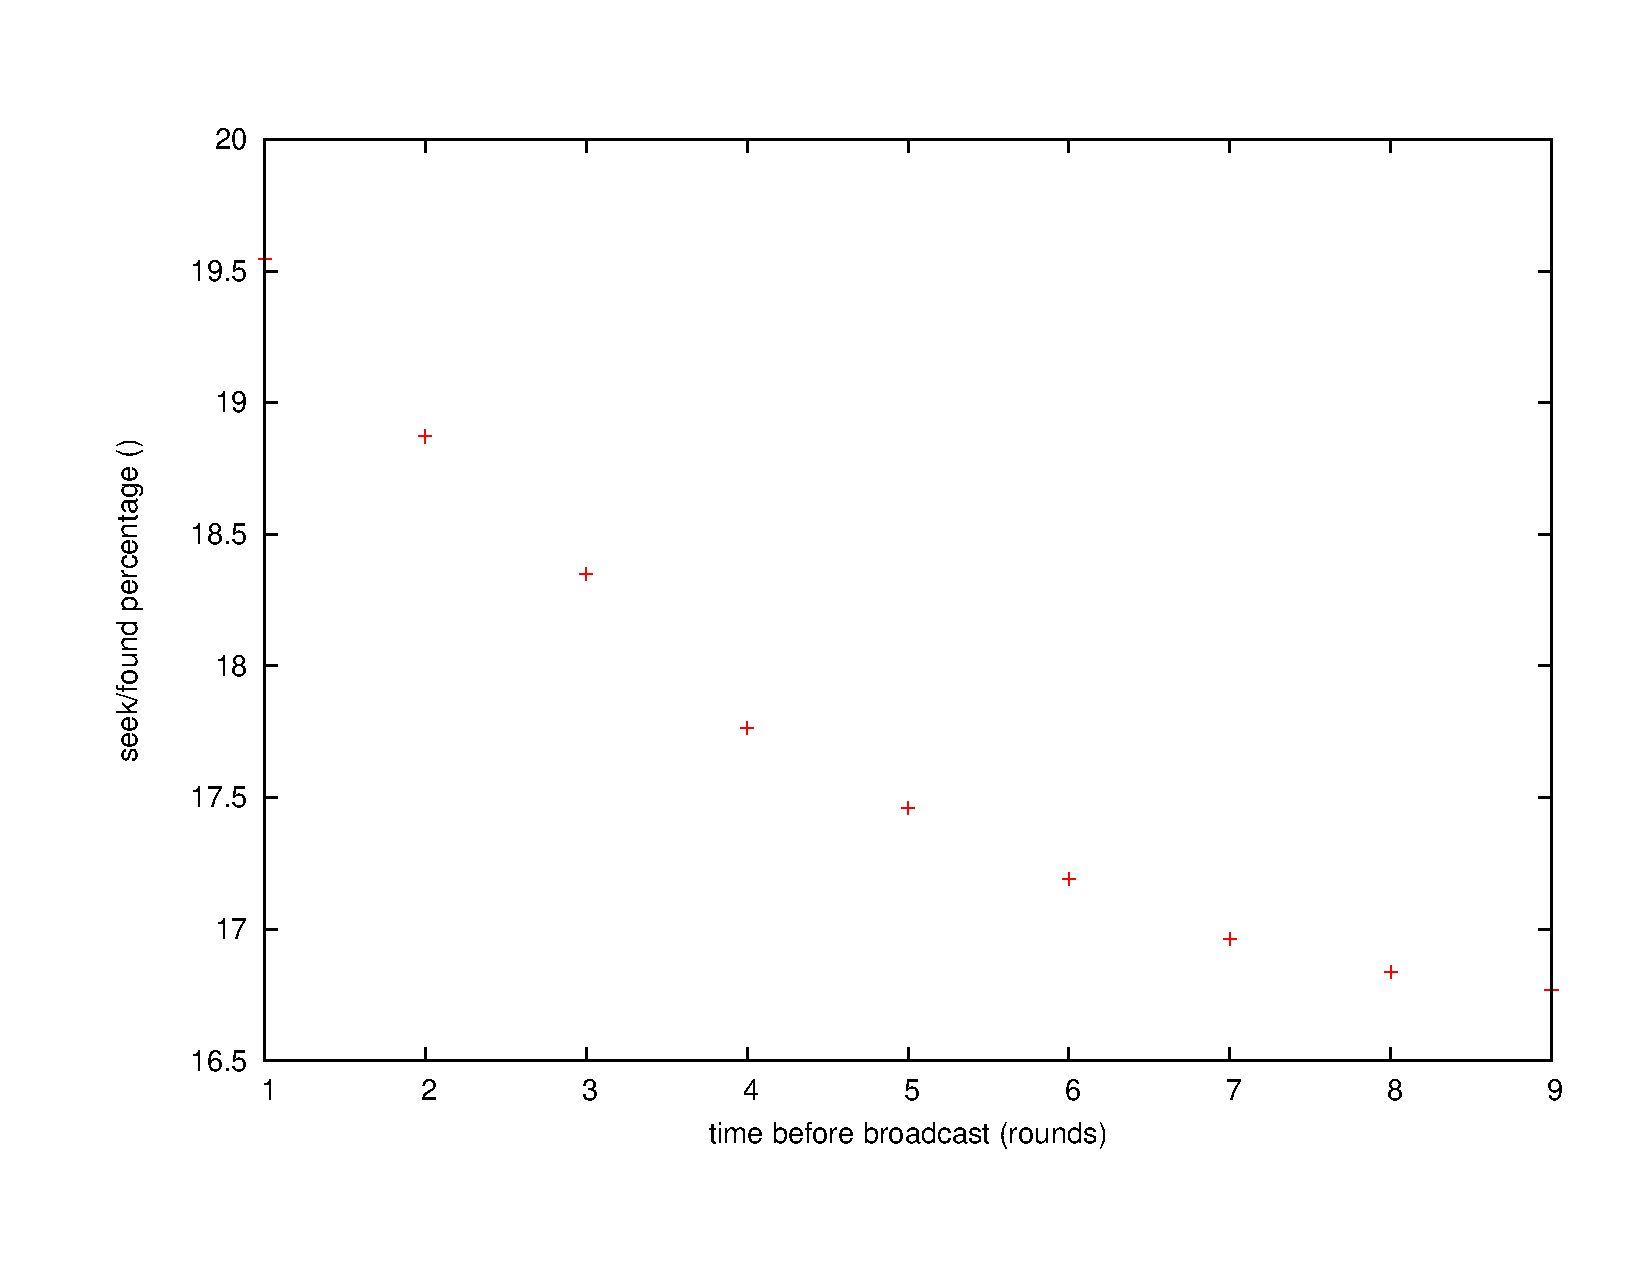
\includegraphics[scale=.3]{src/timeb4broad-seekfound}
      \label{timeb4broad:seekfound}
    }
    
    \subfigure[Ratio temps garé / temps total]{
      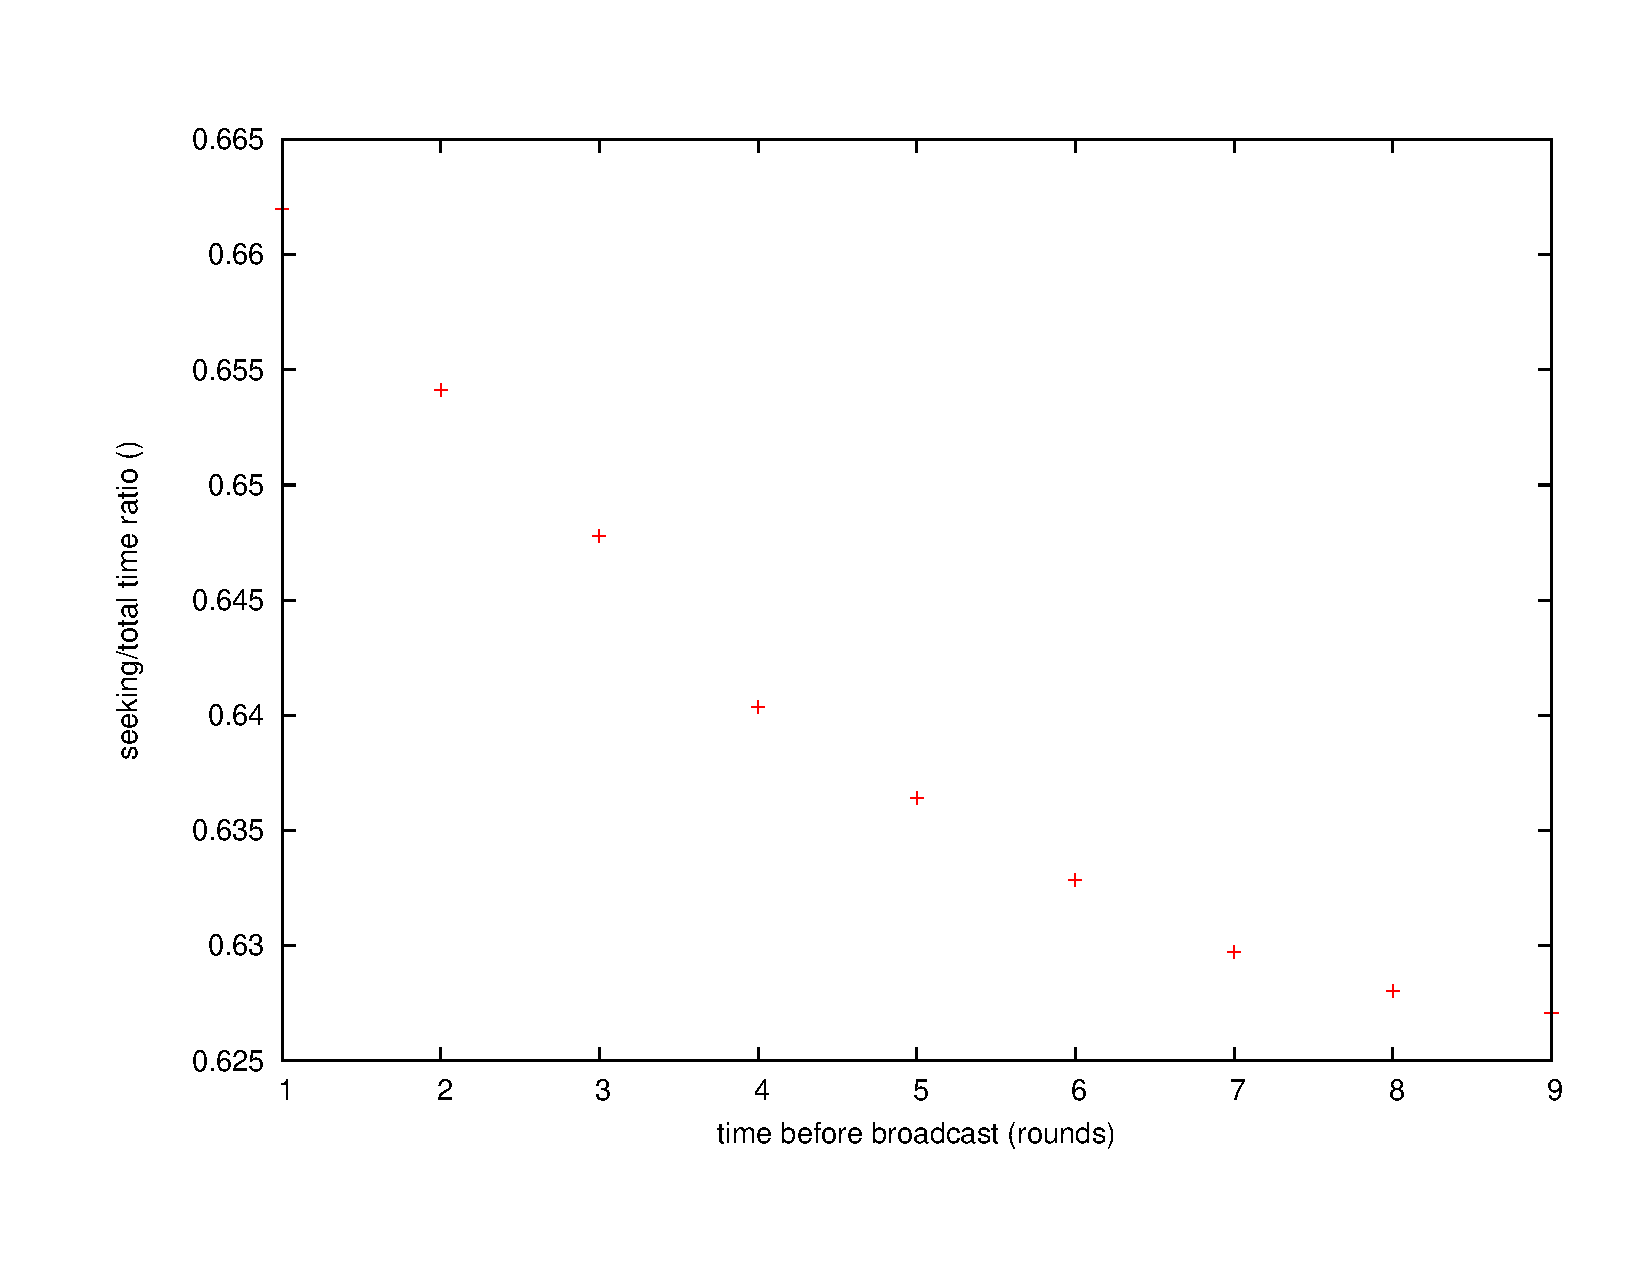
\includegraphics[scale=.3]{src/timeb4broad-seeking}
      \label{timeb4broad:seeking}
    }
  \end{center}

  \caption{Résultats obtenus en faisant varier le temps avant diffusion}
  \label{timeb4broad:all}
\end{figure}

\subsubsection{Variation du temps avant recherche}

Finalement, le dernier paramètre local à notre système est le temps qu'un agent met avant de se remettre à la recherche d'une place après en avoir quitté une. C'est ce qu'on peut appeler un paramètre d'équité, il est censé assurer qu'aucun agent ne monopolise de ressources.

\paragraph{Résultats et interprétation}

Les résultats sont présentés dans la figure \ref{timeb4search:all}\\

C'est le paramètre qui donne les résultats les plus intéressants. Tout d'abord le nombre de messages augmente linéairement par rapport au temps avant une nouvelle recherche. En effet, plus les agents s'éloignent de leur position de stationnement, plus ils vont explorer le terrain et donc trouver d'autres places.\\

Les deux courbes de ratios montrent une forme non rencontrée jusqu'à présent. Les solutions locales et globales commencent par se détériorer pour s'améliorer de manière remarquable. Cela s'explique en comprenant que les faibles valeurs provoquent un phénomène d'appropriation des places qui reviennent toujours au même agent. Les fortes valeurs elles correspondent à une équité forte, les agents s'éloignent suffisamment de leur ancienne place pour ne plus retourner dessus tout de suite après laissant la place à un autre agent. La perte de performance est du à un éloignement fort provoquant une perte de temps pour retourner sur la place mais trop faible pour qu'un autre agent ou une autre place soit trouvé.\\

Finalement, plus les agents se dispersent sur la grille meilleur sont les solutions locales et globales. Ceci se payant malheureusement par un fort nombre de messages échangés.

\begin{figure}
  \begin{center}
    \subfigure[Nombre de messages en fonction du temps avant une nouvelle recherche]{
      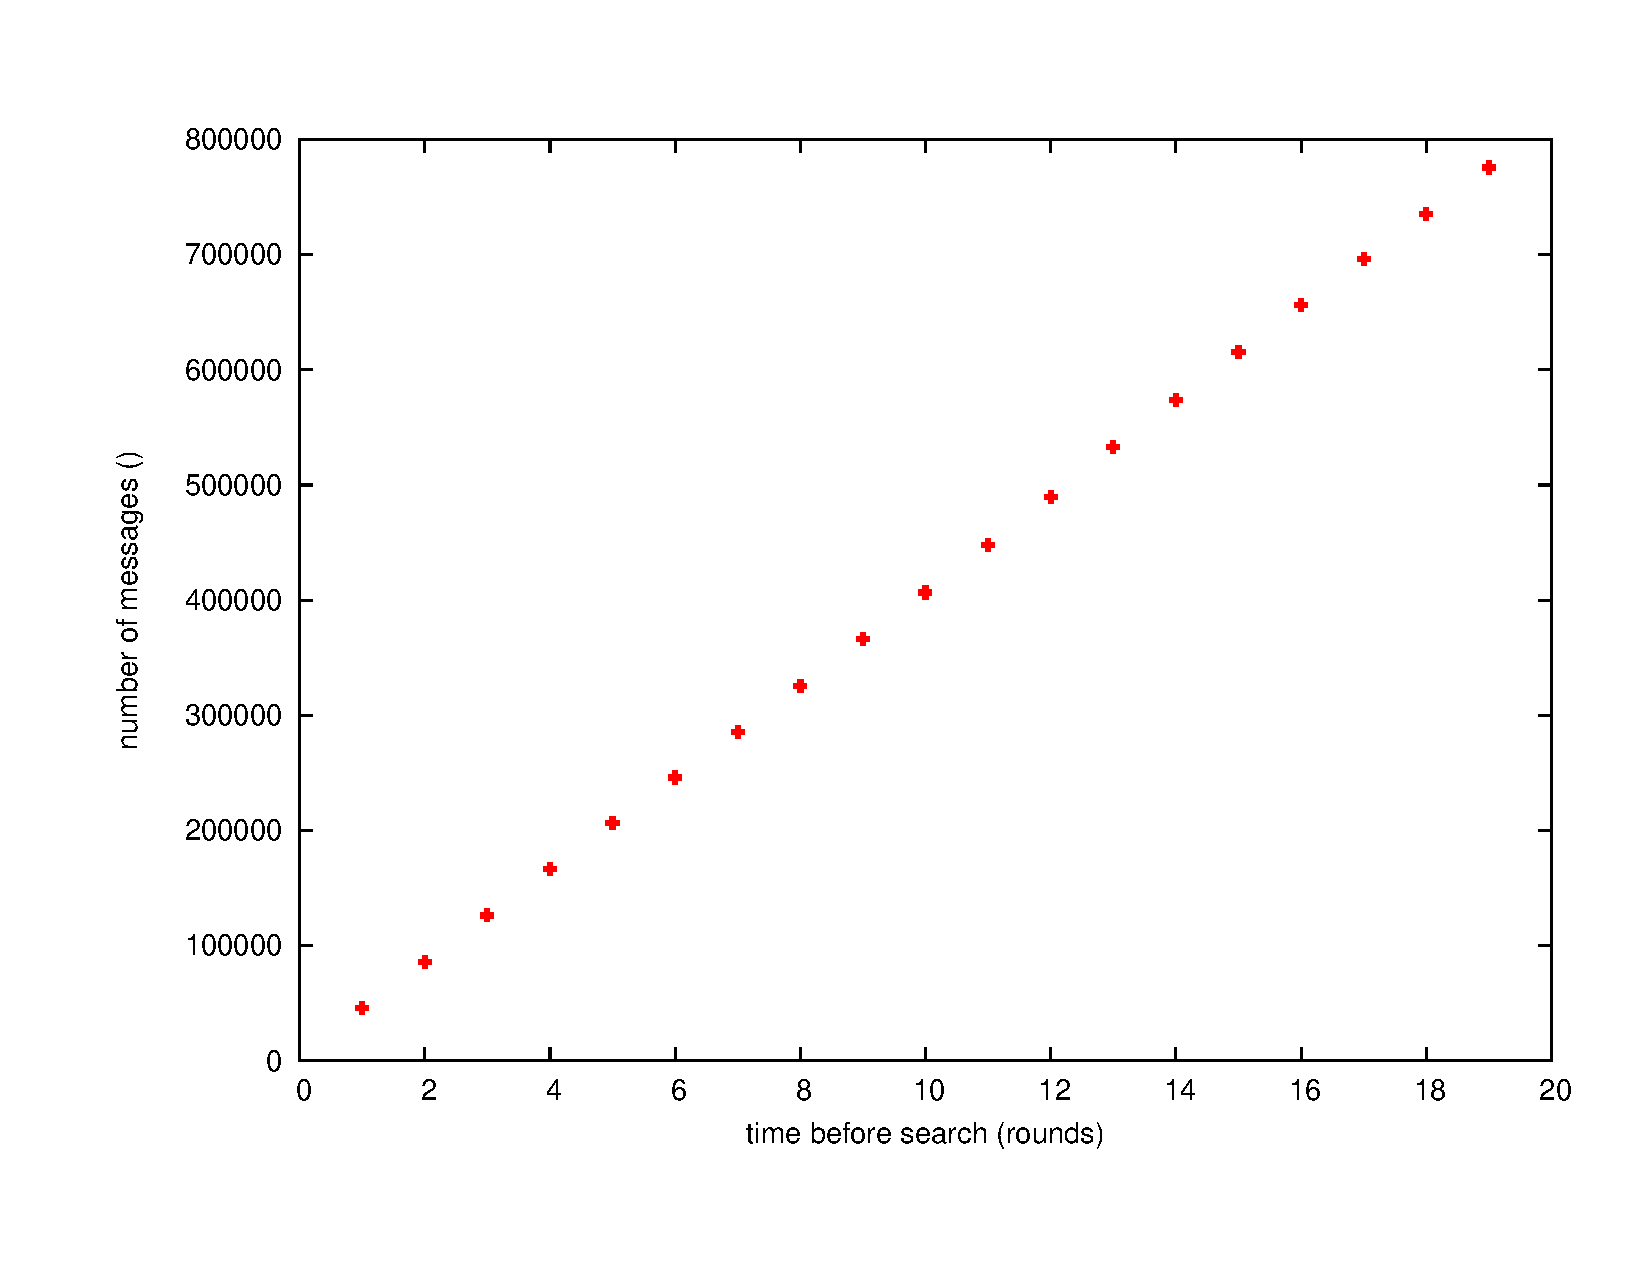
\includegraphics[scale=.3]{src/timeb4search-message}
      \label{timeb4search:message}
    }
    
    \subfigure[Pourcentage temps de vagabondage / temps vers place]{
      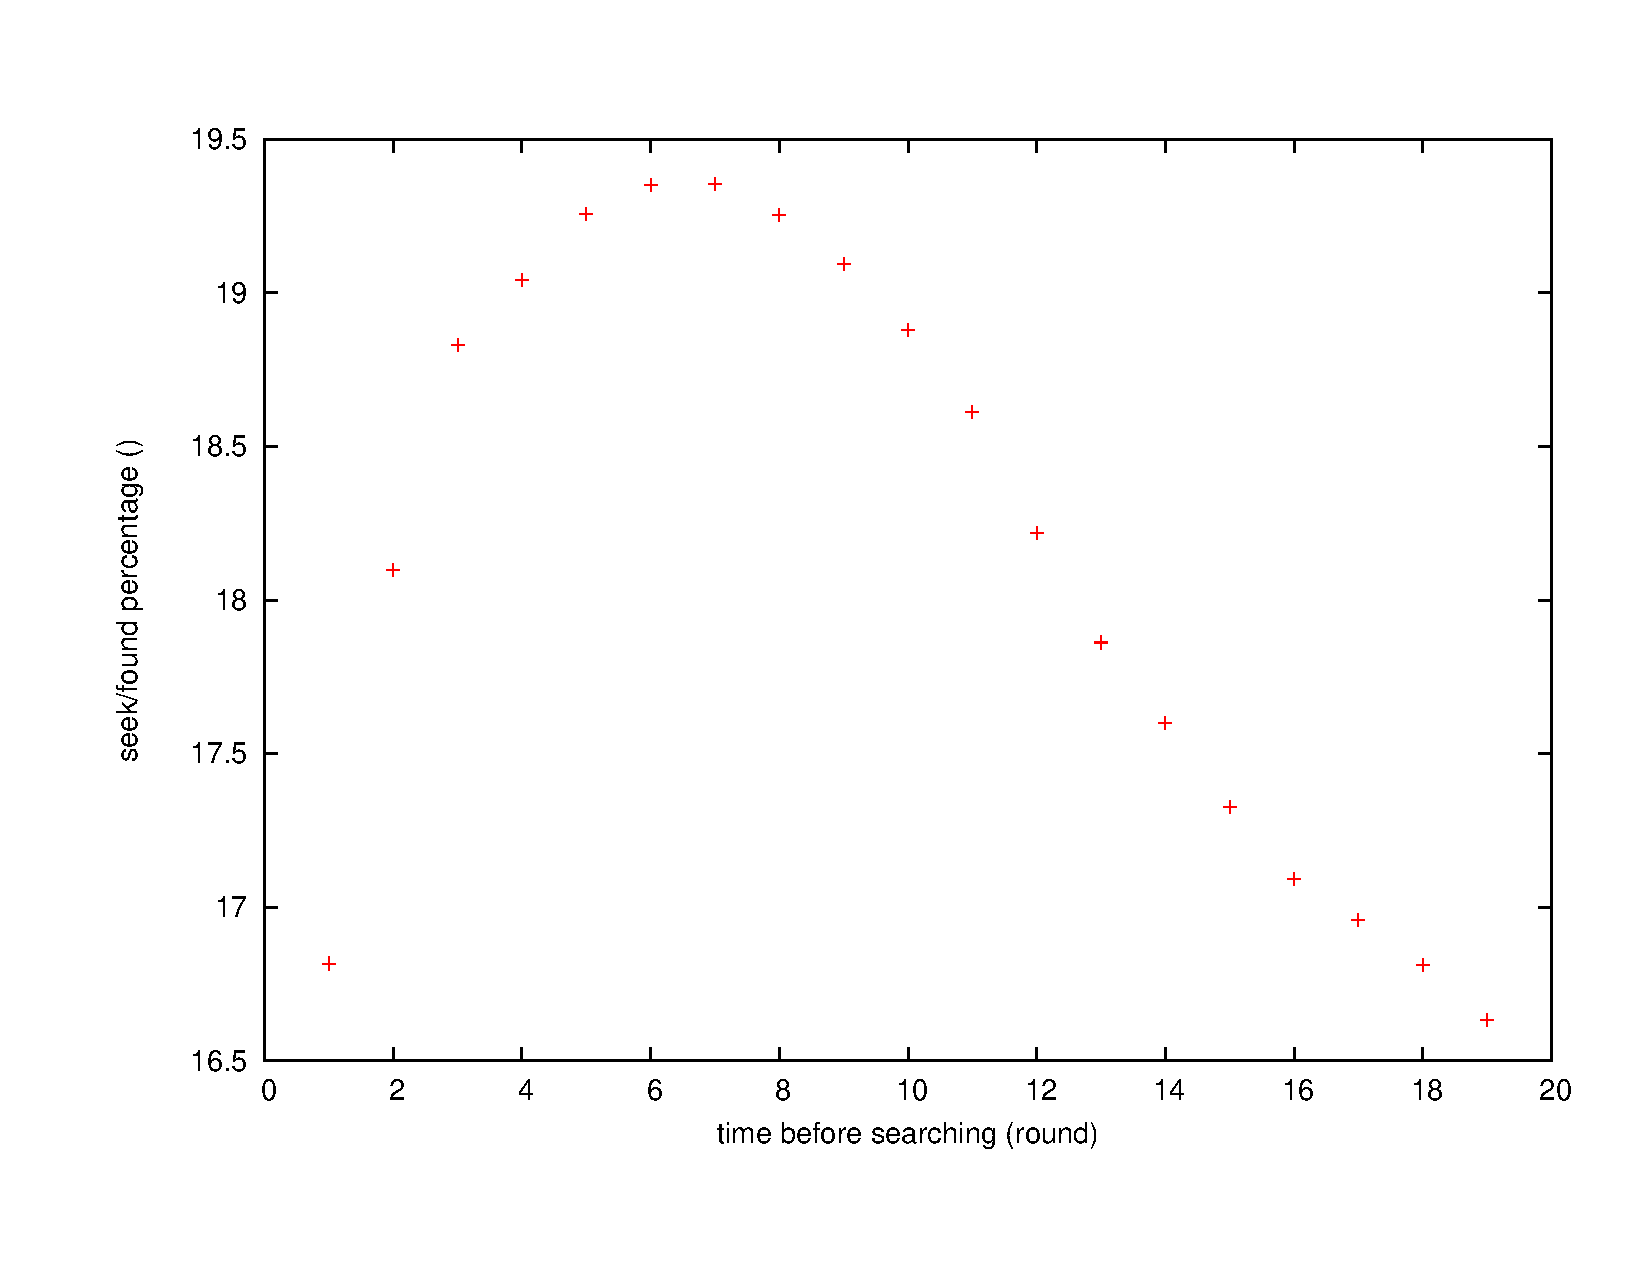
\includegraphics[scale=.3]{src/timeb4search-seekfound}
      \label{timeb4search:seekfound}
    }
    
    \subfigure[Ratio temps garé / temps total]{
      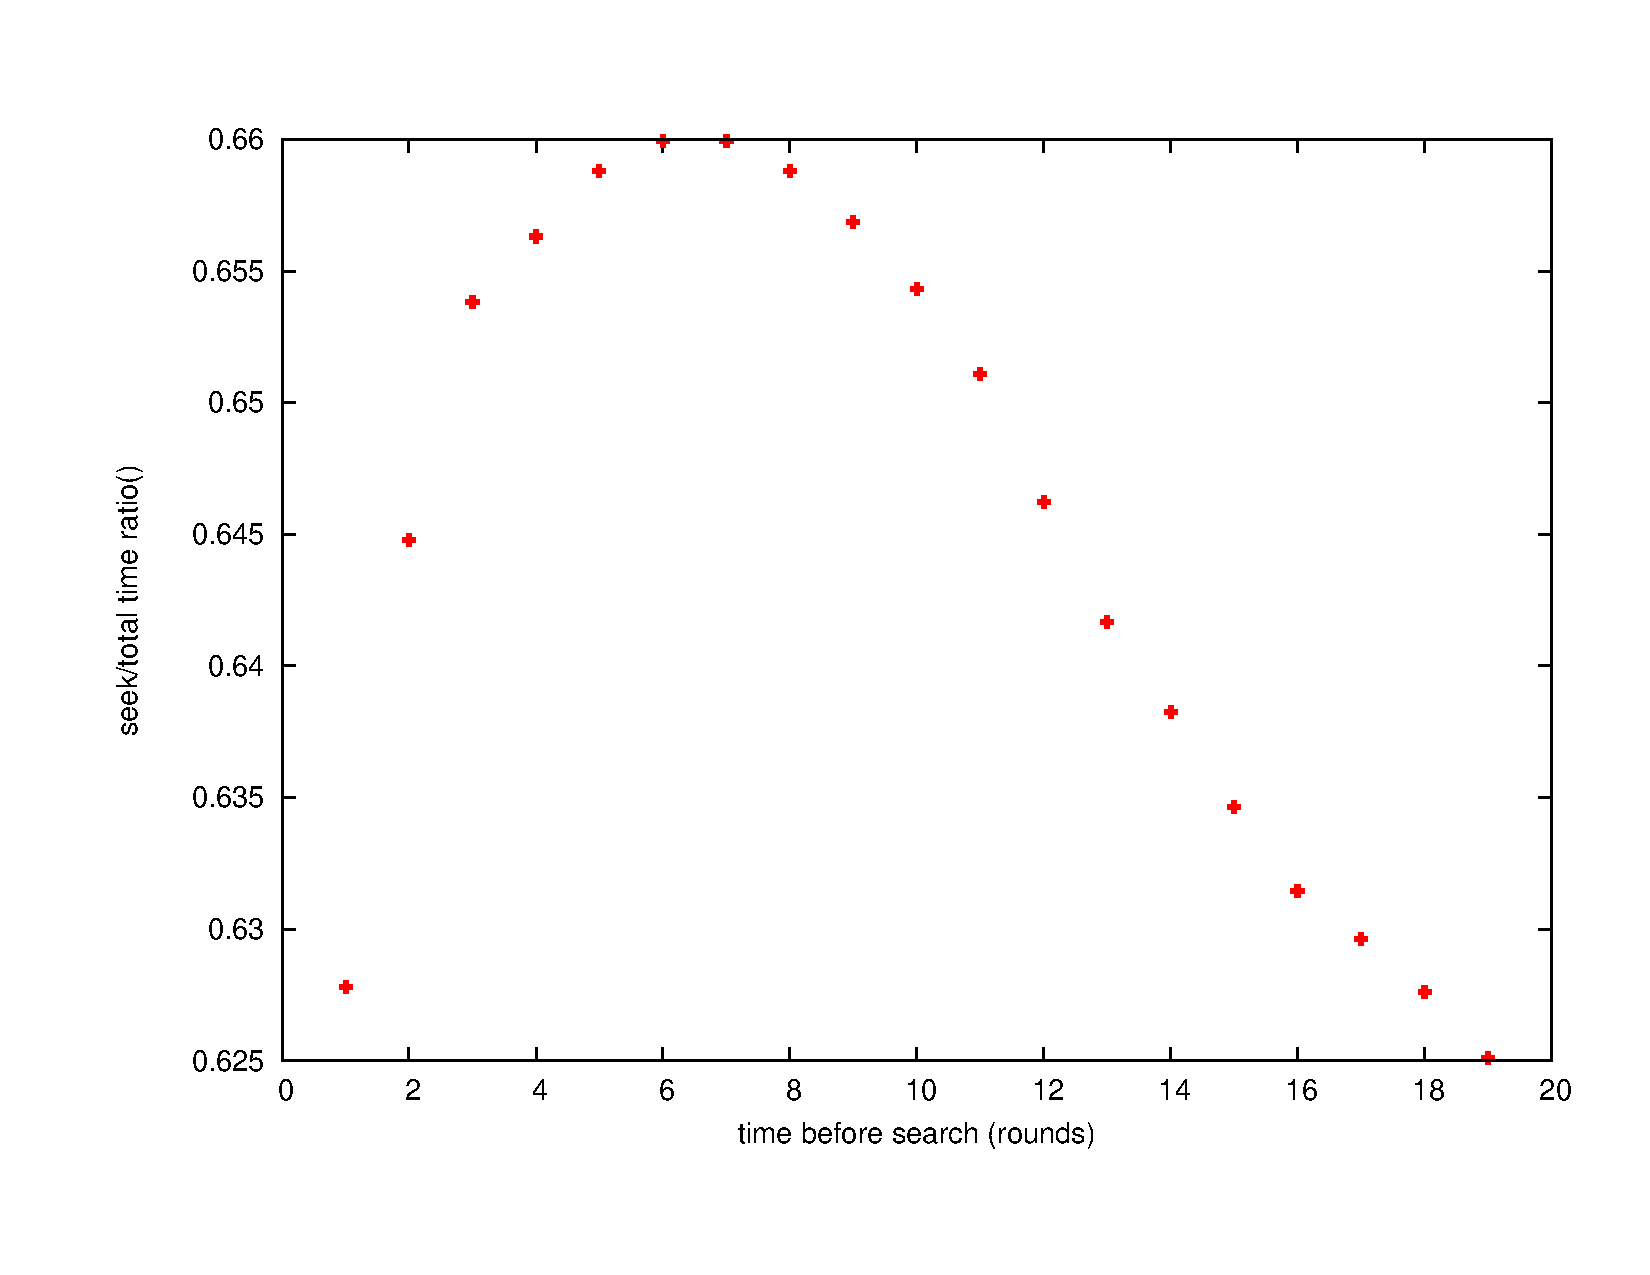
\includegraphics[scale=.3]{src/timeb4search-seeking}
      \label{timeb4search:seeking}
    }
  \end{center}

  \caption{Résultats obtenus en faisant varier le temps avant une nouvelle recherche}
  \label{timeb4search:all}
\end{figure}

\subsection{Paramètres du système}

Cette fois nous faisons varier le nombre d'agents et le nombre de places disponibles. La seule contrainte étant qu'il y aille toujours moins de places que de voitures.

%%% Local Variables:
%%% mode: latex
%%% TeX-master: "../sma"
%%% compile-command: "cd ..; make"
%%% End:
